%------------------------------------------------------------------------------%
%                                   cholesky                                   %
%------------------------------------------------------------------------------%

\section{Cholesky}

\gls{fds}'s simulation requires to solve equations. For this they are able to
use the Cholesky algorithm, however, their current implementation is not fast
enough. In this section, we will start by presenting the algorithm. Then we
will explain the implementation with \gls{hh} before presenting the results. For
the measures, our implementation will be compared to the openblas's one as it is
one of the fastest currently available.

\subsection{The algorithm}
\label{sec:choalgo}

The Cholesky algorithm is used to solve systems of linear equations of the form
$Ax = y$ where $A \in M_{n,n}(\mathrm{R})$ is symmetric and positive-definite
\cite{choleskywiki}. The principle is to decompose the matrix $A$ into a matrix
$L$ such as $A = LL^{T}$ where $L \in M_{n,n}(\mathrm{R})$ is a lower triangular
matrix. Then, we can solve the two sub-problems: $Lx' = y$ and $L^{T}x = x'$.

There are several ways to implement this algorithm. Here, we are going to
implement the block version since it is the most adapted to parallel computing.
Indeed, one most important notions of \gls{hpc} is the optimization of the CPU
cache usage. To do this, we will decompose our matrix into smaller blocks that
can be entirely loaded into the cache in order for the CPU not to access the
RAM.

The version of the algorithm that we will use is explained by
\cite{choleskyblock}. This algorithm is done in three steps. First, let's
consider the matrix $A$ visible on the figure \ref{fig:chodeca}. On this figure,
$D$ is a diagonal block, $C$ is a column (composed of multiple blocks) and $A'$
is a sub-matrix.

% [Cholesky decomposition] {{{
\begin{figure}[h!]
  \begin{center}
    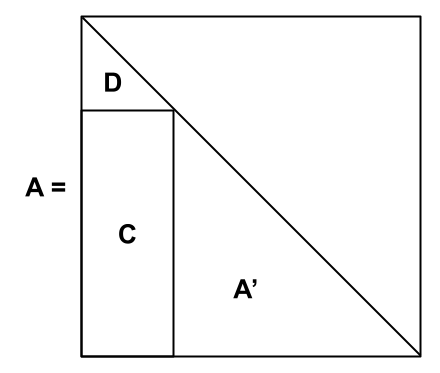
\includegraphics[scale=0.4]{img/cho_block_dec_A.png}
    \caption{Cholesky decomposition: matrix A}
    \label{fig:chodeca}
  \end{center}
\end{figure}
%}}}

The first step of the algorithm is to treat the diagonal element $D$. To do
this, we use the sequential version of the algorithm. It will be fast enough
considering the size of the block. The second step is to update the elements on
the column beneath the diagonal block. To do this, we solve the system $C_{new}
= C(D^{T})^{-1}$. Once it is done, we have computed the first column of the
result matrix $L$. The last step consists of updating the rest of the matrix $A$
by doing $A' = A' - CC^{T}$.

Once we have obtained the matrix $L$, we can proceed to the solving part to find
the solutions of the system. It can be decomposed in two steps: first, we solve
the equation with the diagonal block, then we update the rest of the matrix
using the partial solution (we remove the variables from the equation). We
repeat these steps for each diagonal blocks to solve a sub-problem. The solver
must be used twice to solve the two sub-systems.

\subsection{Implementation}

The implementation of the algorithm has been done in two parts. The
decomposition as been done first, and once it was fully functional, the solver
part has been added. This choice has been made because the decomposition is the
most critical piece of the algorithm. It was important to compare our version
with the openblas's one before implementing the solver.

The first implementation of the decomposition consisted of the creation of a
graph that followed the steps describe in the section \ref{sec:choalgo}
similarly to openblas. This graph is visible on the figure \ref{fig:chograph}.

%todo: graph
% [Cholesky decomposition graph] {{{
\begin{figure}[h!]
  \begin{center}
    \includegraphics[scale=0.2]{img/cho_graph.png}
    \caption{Cholesky decomposition graph}
    \label{fig:chograph}
  \end{center}
\end{figure}
%}}}

%todo: explain the tasks
%todo: explain data

This first solution was too slow since we were executing the three steps
sequentially (this is also what is done in openblas). By doing so, we were
loosing a lot of parallelism. For instance, the computation of the diagonal
elements could be done with only one thread and all the other threads had to
wait. To optimize the algorithm, we wanted to keep the threads as busy as
possible and the solution for this was to rely on early computation by
processing the blocks as soon as they are ready. For instance, we can start
solving the next diagonal element before all the blocks of the sub-matrix $A'$
are updated. We can do the same thing with the column blocks.

To make the early computation possible, the block's data structure has been
changed. A \texttt{rank} attribute has been added to keep track of the
modifications on the blocks. Each time a block is updated, its rank is
increased. When the rank of a block is equal to its column number, it is ready
to be processed, and it is processed when its rank is superior to its column
number. The states use pending lists to store indices of blocks that should be
processed, and iterate on these lists to launch the computation of all ready
blocks.

In this second version, there are a lot of verifications to make, using the rank
in the states. Furthermore, both of the states have a vector of block pointers
that are shared between them to make sure that when the \textit{decompose state}
changes a rank, the \textit{update state} can be aware of the modification
directly, without any notification. This improves the performances but adds more
complexity in the states.

Eventually, we managed to have good performances with this second version
openblas does not make any early computation. We will describe our results in
the section \ref{sec:chores}.

For the solver, we have a second graph that we use twice to solve the two
sub-system of the matrix. The graph can be seen on the figure
\ref{fig:solvergraph}.

%todo: solver graph
% [Solver graph] {{{
\begin{figure}[h!]
  \begin{center}
    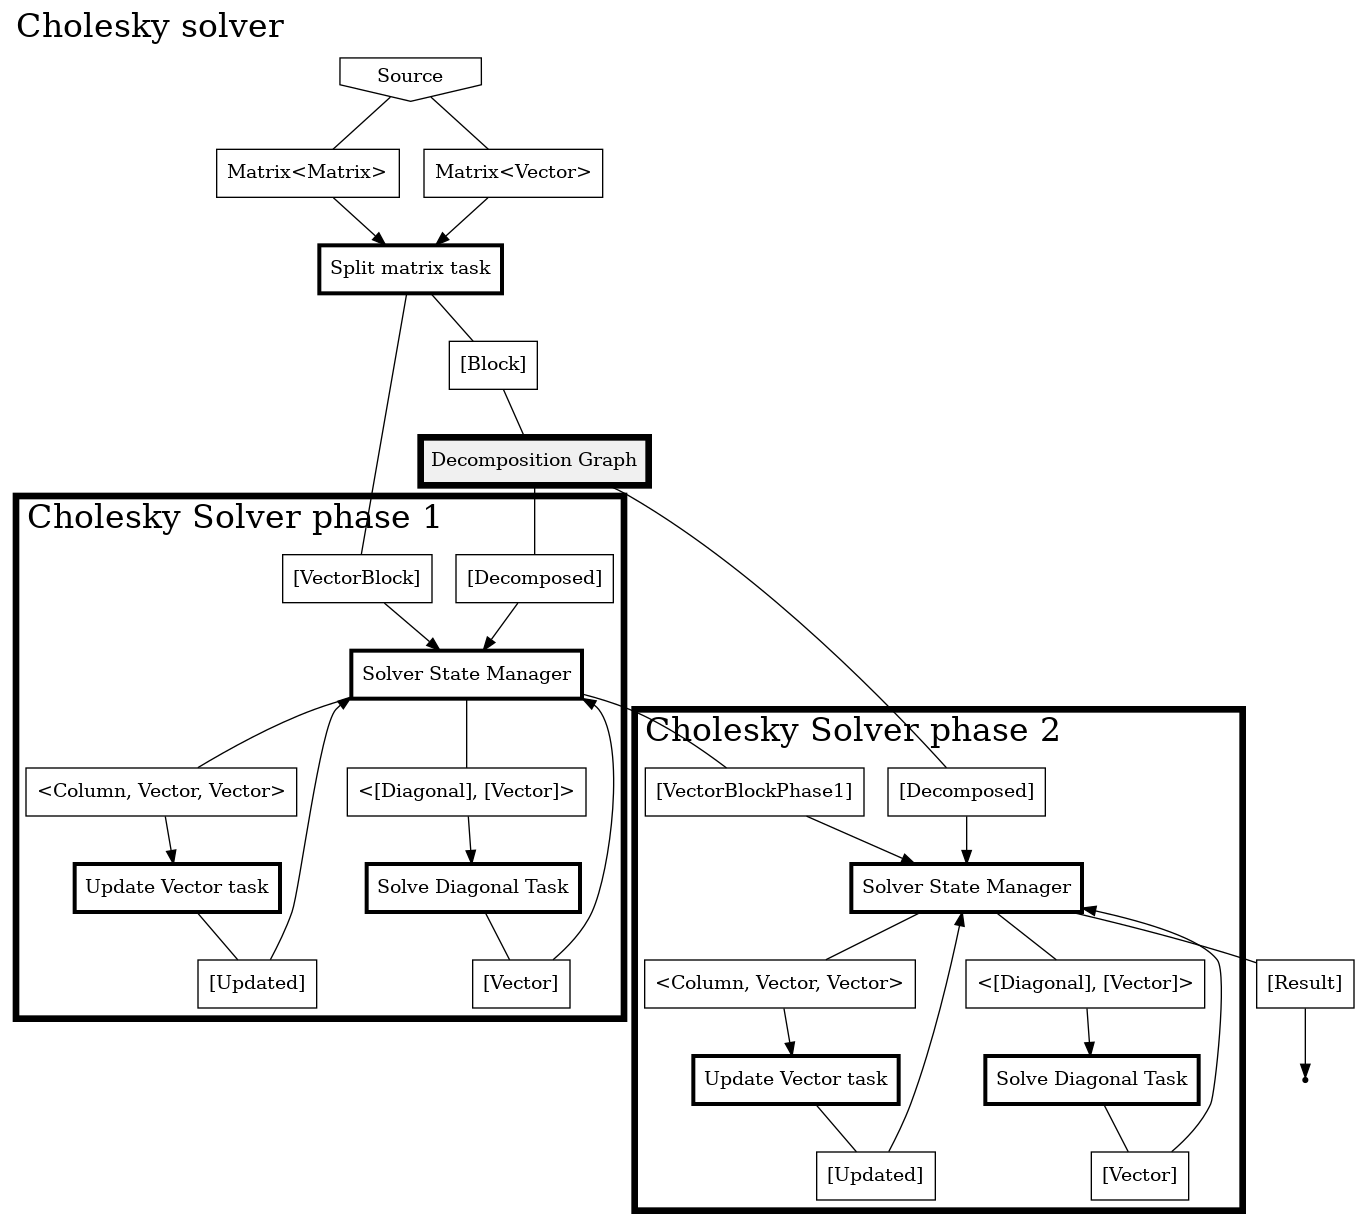
\includegraphics[scale=0.2]{img/solver_graph.img}
    \caption{Solver graph}
    \label{fig:solvergraph}
  \end{center}
\end{figure}
%}}}
%todo: explain the solver graph

In this graph we use the same matrix blocks as in the decomposition graph, so
we can start the solving directly when the blocks are decomposed. The hole
principle of \gls{hh} is to allow the creation of pipelines in which the data
flow continuously, so we do not have any barrier between the tasks. Here, we do
not have to finish the decomposition entirely to start solving the blocks. This
helps keeping as much parallelism as possible and always use the biggest amount
of the computer's resources. In other words, if we represented the computation
time between the logical cores in a Gantt diagram, we would like to optimize the
overlap between tasks and have as little gaps as possible (the cores should
not be in a wait state for too long, at all ideally).

\subsection{The results}
\label{sec:chores}
